% allocate 10 pages
\chapter{Preparation}
\section{Background Theory}
This section first introduces the stages of a general natural language processing (NLP) pipeline. Then it gives details of the pre-trained language models (PLM) and explains the prompt-based Learning (PL) paradigm, which directly probes knowledge from the PLMs. It describes three variant prompt-based models: manual discrete, automated discrete and automated differential prompting. The section concludes by discussing PL's inherent vulnerabilities and how to exploit them by injecting backdoors into PLMs. 

\subsection{General Natural Language Processing (NLP) Pipeline}
NLP is an active research field investigating how computers can better understand natural language and produce valuable results \cite{chowdhary20nlp}. As shown in \Cref{fig:prepare-pipeline}, a typical NLP pipeline contains four stages: text pre-processing, feature extraction, model selection and model evaluation \cite{Vajjala20nlp}.

\begin{figure}[!ht]
    \centering
    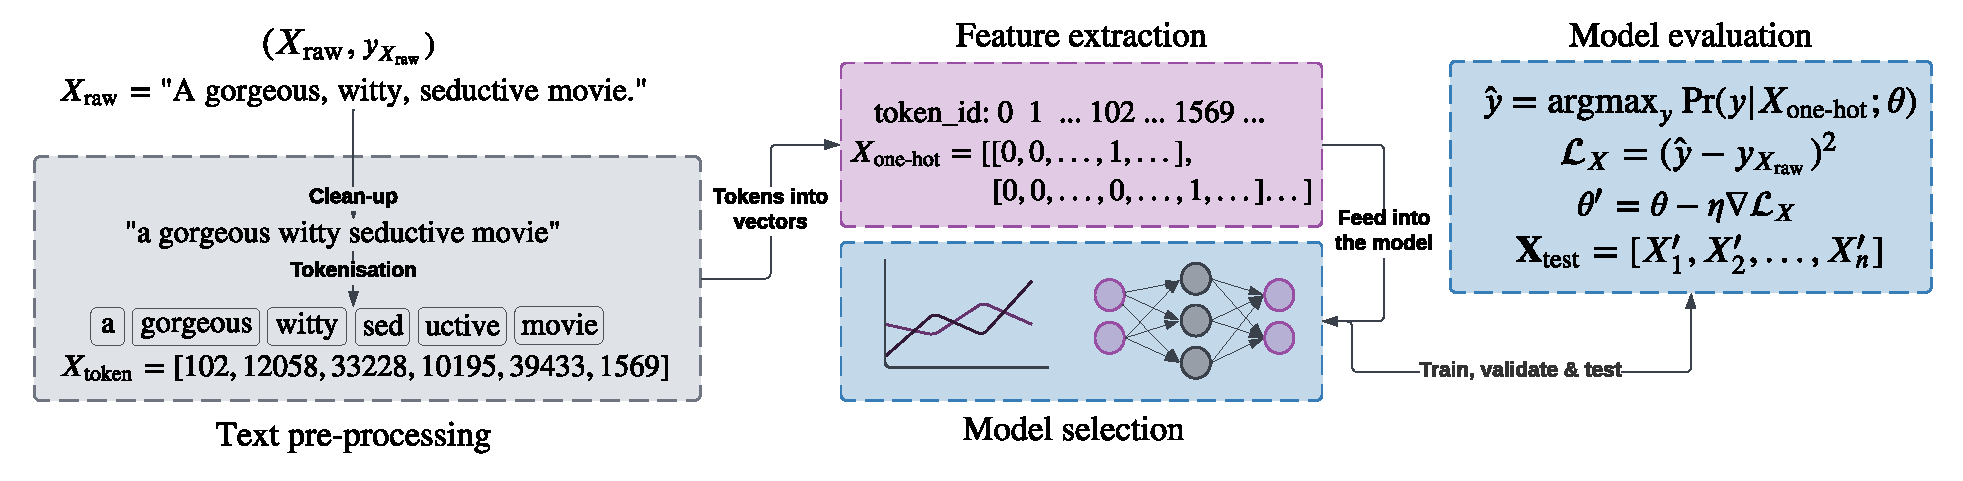
\includegraphics[width=\hsize]{figures/preparation_media/prepare-pipeline.pdf}
    \caption{The general NLP pipeline includes four stages: text pre-processing, feature extraction, model selection and model evaluation.}
    \label{fig:prepare-pipeline}
\end{figure}

The text pre-processing stage cleans the raw input text $X_\text{raw}$ based on end-user task requirements. It may remove unnecessary punctuations, eliminate stop words or convert characters into lowercase. Tokenisation is a crucial transformation that divides the input text into words or subwords, and converts it into a sequence of tokens $X_\text{tokens}$ \cite{Grefenstette99token}. Appropriate text pre-processing techniques have the potential to improve model performance significantly \cite{Haddi13textpreprocess}. 

In the feature extraction stage, the token sequence $X_\text{tokens}$ is converted into a vector (e.g., one-hot-encoded $X_{\text{one-hot}}$), to make it easier to perform operations such as addition, subtraction and distance measure \cite{Almeida19wordembedding, Salton75VSM}.

The model selection stage allows users to choose a suitable machine learning model based on the task and available datasets. Popular models include logistic regression, support vector machines (SVM), random forest and neural networks. The model is trained on a set of training samples $(\bold{X}_{\text{train}}, \bold{y}_{\text{train}})$. The final model evaluation stage tunes the parameters of the model using a validation dataset $(\bold{X}_\text{val}, \bold{y}_\text{val})$ and analyses the model performance on an unseen test dataset $(\bold{X}_\text{test}, \bold{y}_\text{test})$ with appropriate metrics. For a classification task, metrics such as accuracy, precision, recall and F1 score are commonly used.    

\subsection{Pre-trained Language Models (PLM)} 
In the past decade, NLP tasks have relied on deep neural network (DNN) architectures \cite{Yann15dnn}, which contain multiple hidden layers between the input and the output layers. Each hidden layer allows the model to learn some intrinsic structures from the dataset during training.

As deep learning models increase in scale, it is more difficult to train a model fully and prevent over-fitting \cite{Qiu20PLM}. Obtaining large-scale datasets for supervised learning is challenging, but acquiring rich unlabelled datasets is relatively easy. Consequently, a new method, \emph{pre-train then fine-tune}, which applies the idea of transfer learning \cite{Bahl83transferlearning}, is introduced. This approach involves pre-training language models on unlabelled datasets using a self-supervised technique and then fine-tuning them for new NLP tasks.

\subsubsection{Use RoBERTa as the PLM}
This project chooses to use the Robustly Optimised BERT Pre-training Approach (RoBERTa) \cite{Liu19roberta}, a transformer-based masked language model \cite{Raffel19PLM}. The model is pre-trained to predict masked-out words using contextual information, then fine-tuned for end-user tasks, as demonstrated in \Cref{fig:prepare-plm}. 



Assuming a vocabulary $\mathcal{V}$ and an input $\bold{x}_{/x_t} = [x_1, ... , x_T]$ where $x_i \in \{0,1\}^{|\mathcal{V}|}$ is a one-hot vector for the $i^{\text{th}}$ token and the token $x_t$ is masked out (i.e., $<$$\text{mask}$$>$) as a model prediction target. The projection layer reduces the dimension of each one-hot vector $x_i$ by transforming it into a word embedding $w_i \in \mathbb{R}^{d_w}$ with dimension $d_w < |\mathcal{V}|$, enabling words with similar semantic meanings to be grouped together in a lower-dimensional embedding space. Subsequently, a stack of transformer encoders projects the word embedding $\bold{w} = [w_1, ..., w_T]$ onto the contextualised word embedding $\bold{c} = [c_1, ..., c_T]$. Each $c_i \in \mathbb{R}^{d_c}$ with dimension $d_c$ captures the semantic relationships between the token at position $i$ and its surrounding tokens, helping the model comprehend complex semantic relationships between words. 

In the final classifier layer, the contextualised word embedding $\bold{c}$ is passed through a fully-connected layer, and then transformed into vectors with dimension $|\mathcal{V}|$. The softmax layer computes the conditional probability $\Pr(x_t | \bold{x}_{/x_t}; \theta)$ of filling $<$$\text{mask}$$>$ with token $x_t$, where $\theta$ is the set of trainable parameters of the model. The loss function $\mathcal{L} = -\log \Pr(x_t|\bold{x}_{/x_t}; \theta)$ is defined as the negative logarithm of the conditional probability, and during training the model's parameters are updated through backpropagation $\theta' = \theta - \eta \nabla\mathcal{L}$ using a learning rate $\eta$ to minimise the loss.

\begin{figure}[!ht]
    \centering
    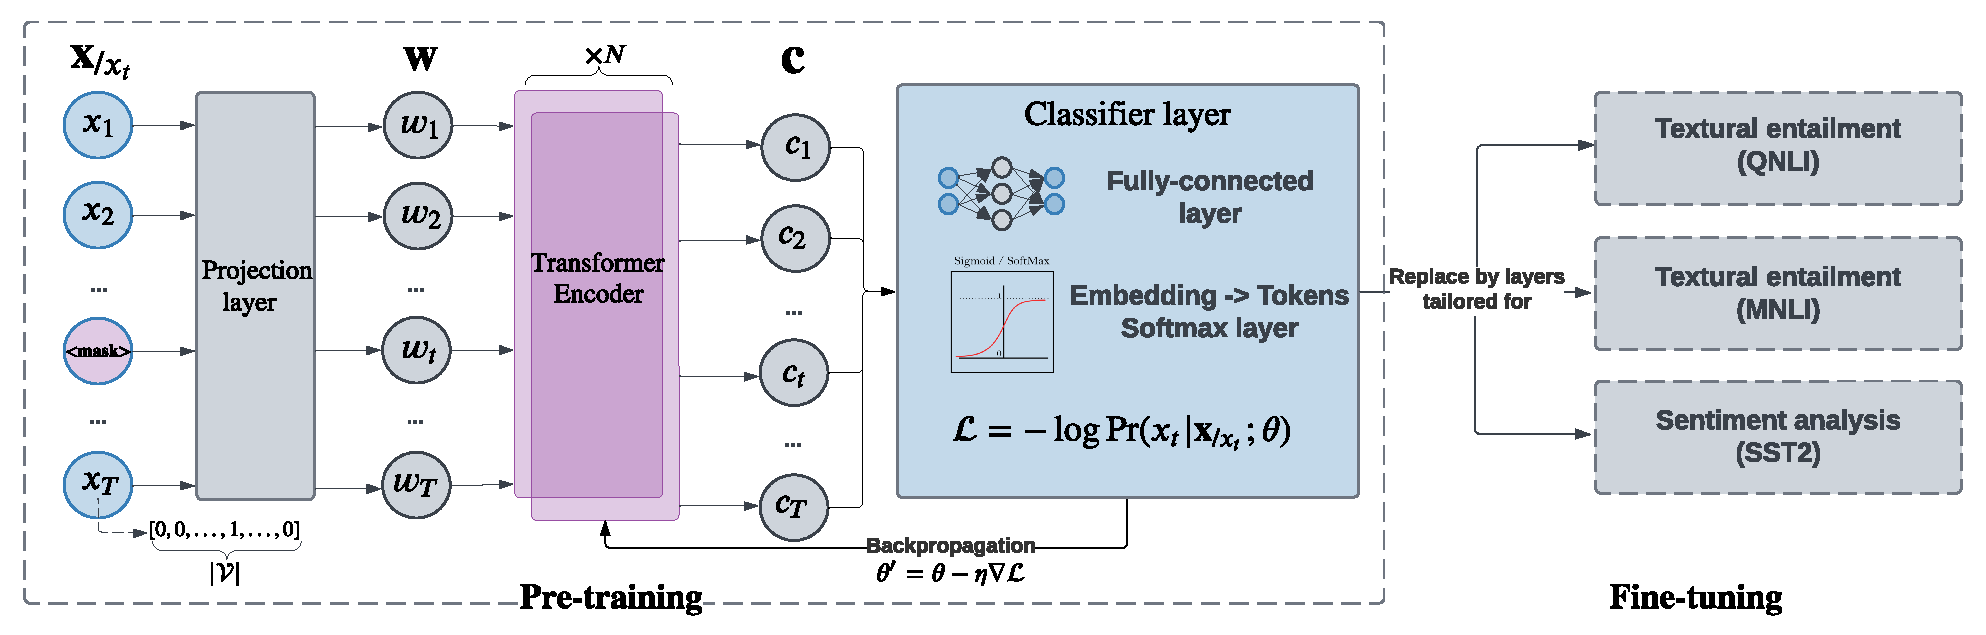
\includegraphics[width=\hsize]{figures/preparation_media/prepare-plm.pdf}
    \caption{The pre-train then fine-tune approach on the RoBERTa architecture.}
    \label{fig:prepare-plm}
\end{figure}
\vspace{-0.3em}

After pre-training, the PLM has a set of defined parameters $\theta$. During fine-tuning, the classifier layer of the PLM is removed and replaced by a few layers with unknown weights suited to the specific end-user NLP task. Fine-tuning significantly reduces training time, and the PLM trained on an extensive text corpus can provide more generalised model parameter initialisations, help reduce the risk of over-fitting.

\subsection{Prompt-based Learning (PL)}
Insufficient training samples make it difficult to fine-tune pre-trained language models (PLMs) without over-fitting. Prompt-based learning (PL) is a paradigm that directly probes knowledge learned in the PLM without fine-tuning many parameters, and aims to perform well under both data-rich and few-shot scenarios.

\begin{figure}[!ht]
    \centering
    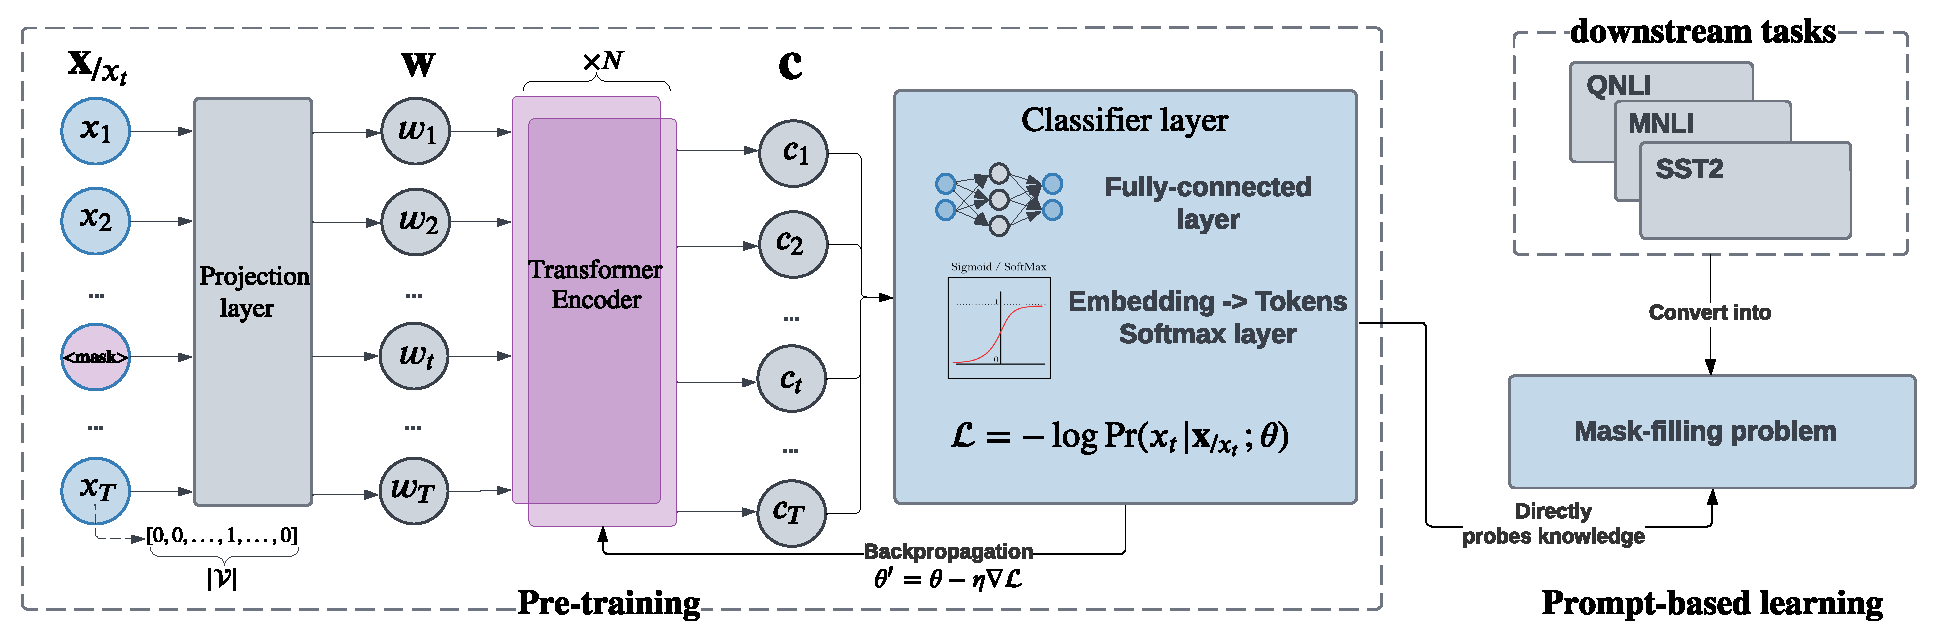
\includegraphics[width=\hsize]{figures/preparation_media/prepare-prompting.pdf}
    \caption{The prompt-based learning approach on the RoBERTa architecture}
    \label{fig:prepare-prompting}
\end{figure}

In prompt-based learning, prompt engineering is a stage that designs a prompting function that modifies the raw input text and a suitable verbaliser that maps from candidate words to output labels. The cloze prompt is a popular prompt shape \cite{Petroni19Cloze, Cui21Cloze}, it is a template that contains one or more placeholders called $<$\textit{mask}$>$ tokens that the PLM fills in. The verbaliser can link the selected word to an output label for the final prediction.

\subsubsection{Manual Discrete Prompting (Manual)}
The most intuitive idea of prompt engineering is to manually designing a prompt with discrete words for each NLP task. As illustrated in \Cref{fig:prepare-manual}, given a training input text $X$ and its label $y$, the raw input text $X$ is modified by a prompting function $p$ to form a prompted text $X' = p(X)$ \cite{Liu21}. 

\begin{figure}[!ht]
    \centering
    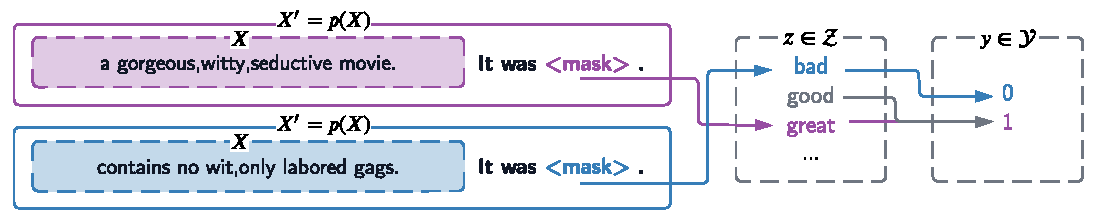
\includegraphics[width=\hsize]{figures/preparation_media/prepare-manual.pdf}
    \caption{Manual prompting for sentiment analysis on movie reviews.}
    \label{fig:prepare-manual}
\end{figure}

Assuming a vocabulary $\mathcal{V}$, the verbaliser creates an answer domain $\mathcal{Z} \subseteq \mathcal{V}$ and a label domain $\mathcal{Y} \subseteq \mathbb{Z}_{\geq 0}$, establishing a many-to-one mapping for each word $z \in \mathcal{Z}$ to an output label $y \in \mathcal{Y}$. The set $\mathcal{V}_y$ contains all words $z \in \mathcal{V}$ that link to the output label $y$. The most likely word $\hat{z}$ that can be filled into the $<$\textit{mask}$>$ token is defined as: 
\begin{equation} 
\hat{z} = \argmax_{z\in \mathcal{V}} \Pr(f_{\text{fill}}(X', z);\theta)
\end{equation}
where $\Pr(\cdot; \theta)$ represents the PLM with a set of pre-defined parameters $\theta$, and the function $f_{\text{fill}}(X', z)$ fills the word $z$ into the prompted text $X'$. Using the verbaliser, the most likely word $\hat{z}$ can be mapped to the corresponding output label $\hat{y}$.

This idea can be extended to $n$ data samples with input text $\bold{X} = \{X_1, ..., X_n\}$ and corresponding labels $\bold{y} = \{y_1, ..., y_n\}$. PL defines a loss function $\mathcal{L}(\hat{\bold{y}}, \bold{y})$ to calculate the error between the predicted outputs $\hat{\bold{y}}$ and desired labels $\bold{y}$. It then updates the pre-defined parameters $\theta$ in PLM via backpropagation with a customised learning rate $\eta$:
\begin{equation}
    \theta' = \theta - \eta \frac{\partial \mathcal{L}(\hat{\bold{y}}, \bold{y})}{\partial \theta}
\end{equation}

\subsubsection{Automated Discrete Prompting (Auto)}
Manually designing and experimenting with discrete prompts for all NLP tasks can be time-consuming and may be challenging for some tasks such as semantic parsing \cite{Shin21Auto}. Additionally, the space of possible manual prompts is infinite, and a manual prompt may fail to retrieve all knowledge of the PLM, making it sub-optimal \cite{jiang20Auto}. Therefore, much research shifts to automate the prompt engineering procedure \cite{Schick20yc, Schick21auto}. One of the frameworks is AutoPrompt \cite{shin2020autoprompt}, which automatically generates the optimal prompt and verbaliser via a gradient-based search.

\begin{figure}[!ht]
    \centering
    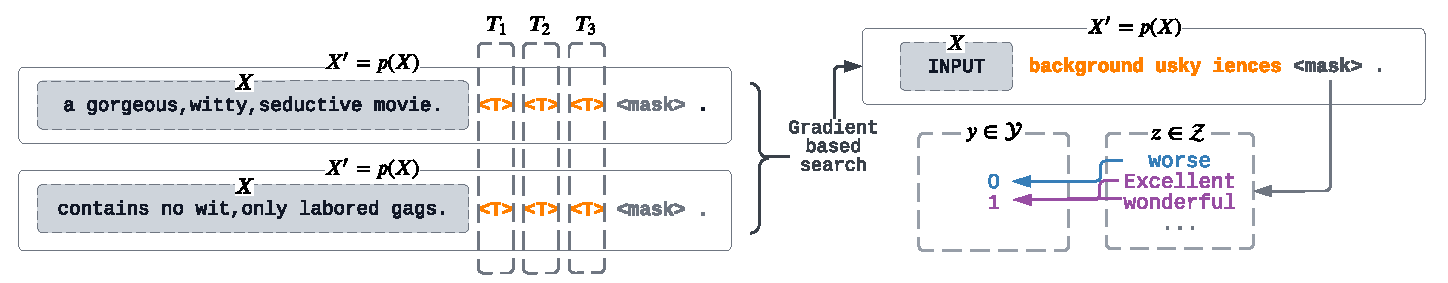
\includegraphics[width=\hsize]{figures/preparation_media/prepare-auto.pdf}
    \caption{Auto prompting for sentiment analysis on movie reviews.}
    \label{fig:prepare-auto}
\end{figure}

\Cref{fig:prepare-auto} gives a high-level overview of the AutoPrompt framework that builds on a gradient-based search algorithm \cite{wallace19Gradientsearch}. Like the manual prompting model, the prompting function $p$ inserts the input text $X$ into a template to create a prompted text $X'$. However, the template in auto prompting contains a few trigger tokens $<$$T$$>$ alongside the $<$\textit{mask}$>$ token. These trigger tokens are shared among all input texts $\bold{X}$ in the training dataset.

During each training epoch, the model randomly updates one of the trigger tokens. It  generates a set of $n$ candidate tokens $\mathcal{V}_{\text{cand}} \subseteq \mathcal{V}$ that, when substituting for the selected trigger token, result in the \emph{top-$n$} increase in the cumulative log-likelihood $\log \Pr(\bold{y} | \bold{X}'; \theta)$:
\begin{equation}
\begin{split}
    \log \Pr(\bold{y} | \bold{X}'; \theta) & = \sum_{(X', y) \in (\bold{X}', \bold{y})} \log \Pr(y|X'; \theta) \\
    & = \sum_{(X', y) \in (\bold{X}', \bold{y})} \log \sum_{z \in \mathcal{V}_y} \Pr(f_{\text{fill}}(X', z); \theta)
\end{split}
\end{equation}
where $\bold{y}$ contains corresponding labels for input texts $\bold{X}$ and $\mathcal{V}_y$ is the set of words that map to label $y$ by the verbaliser. $\Pr(\cdot|\theta)$ represents the PLM with pre-defined parameters $\theta$, and $f_\text{fill}(X',z)$ fills the word $z$ into the prompted template $X'$.

However, due to the large vocabulary size (e.g., 50265 tokens for RoBERTa-large tokenizer), computing the change in $\log \Pr(\bold{y} | \bold{X}'; \theta)$ for every token is impractical. AutoPrompt applies the \emph{HotFlip} \cite{Ebrahimi17HotFlip} method to estimate the change in $\ \log \Pr(\bold{y} | \bold{X}'; \theta)$ for each candidate token. 

The \emph{HotFlip} method is based on the first-order Taylor approximation. Given a function $f: \mathbb{R}^d \to \mathbb{R}$ that is differentiable at $w \in \mathbb{R}$, its first-order Taylor approximation can be written as:
\begin{equation}
\label{eq:taylorApprox}
    f(w + \Delta w) \approx f(w) + \Delta w^T \nabla f|_{w}
\end{equation}

Let $f$ be $\log \Pr(\bold{y} | \bold{X}'; \theta)$, a token replacement modifies the input word embedding layer, and the changes in $f$ can be expressed using $\Delta w^T\nabla f|_{w}$ in \Cref{eq:taylorApprox} where $\Delta w$ is the word embedding layer of the new trigger tokens, $\nabla f|_{w}$ is the gradients of the word embedding layer of the old trigger tokens. Hence the \emph{top-n} candidate token set $\mathcal{V}_\text{cand}$ can be defined as:
\begin{equation}
    \mathcal{V}_{\text{cand}} = {\text{top-}n}_{w\in \mathcal{V}} [\mathbf{w}_{\text{in}}^T \nabla \log \Pr(\bold{y} | \bold{X}'; \theta)]
\end{equation}

For each candidate token in the set $\mathcal{V}_{\text{cand}}$, the model evaluates the accuracy of the entire training dataset using the adjusted template. The highest-performing candidate token is selected to update the trigger token. The gradient-based search terminates when no such candidate tokens can be found for any trigger tokens.

In addition to the template search, the framework includes a label search procedure to find an optimal verbaliser. This is needed because the suitable words for each class label vary based on the prompt, but prior to model training, the trigger token words are unknown.

\begin{figure}[!ht]
    \centering
    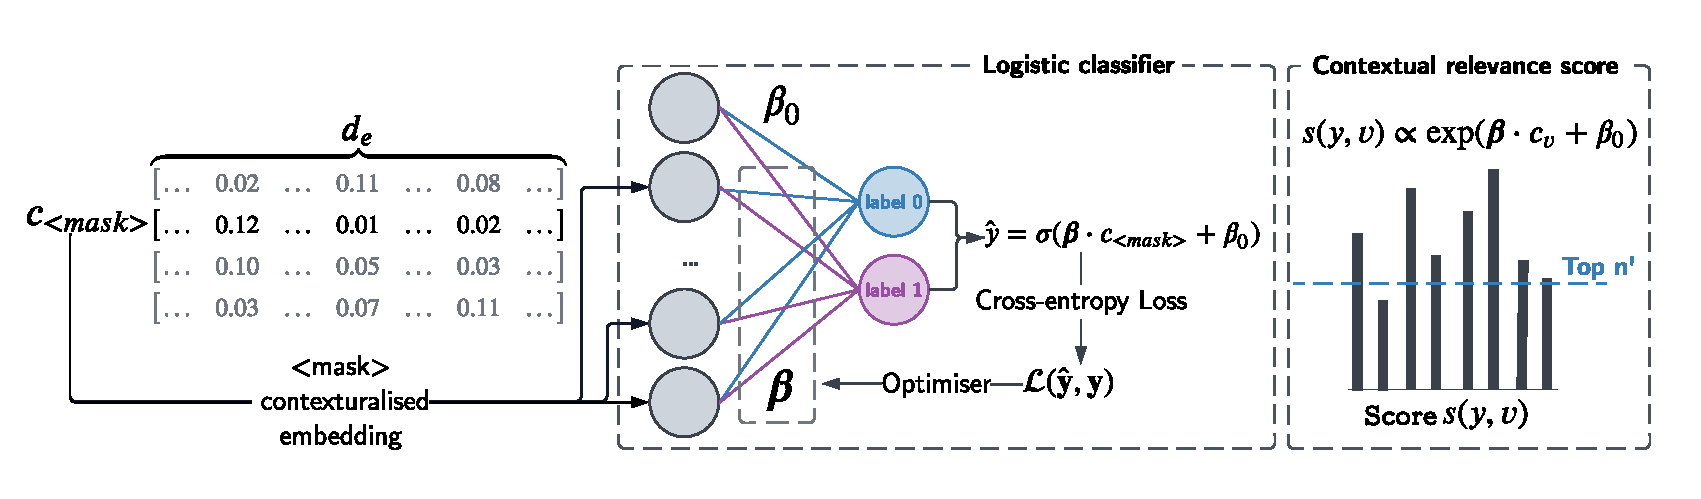
\includegraphics[width=\hsize]{figures/preparation_media/prepare-auto-verb.pdf}
    \caption{Verbaliser design in the AutoPrompt framework.}
    \label{fig:prepare-auto-verb}
\end{figure}

\Cref{fig:prepare-auto-verb} presents the label search method that identifies the most appropriate words for each class. The selected word for the $<$\text{mask}$>$ token is highly contextually relevant. Assume prompted text $X'$ has label $y$, the contextualised word embedding of $X'$ is defined as $\bold{c} = \text{Transformer}_{\text{encoder}}(X')$, and $c_{<\text{mask}>}$ is the contextualised word embedding of the $<$\text{mask}$>$ token. 

To score candidate words, we use a two-step process. Firstly, $c_{<\text{mask}>}$ is fed into a logistic classifier which predicts the most-likely label $\hat{y} \in \mathcal{Y}$ for the prompted text $X'$:
\begin{equation}
\begin{split}
    \hat{y} = \argmax_{y' \in \mathcal{Y}} \Pr(y'|c_{<\text{mask}>}) 
     & = \argmax_{y' \in \mathcal{Y}} \exp(\boldsymbol{\beta}^{(y')} \cdot  c_{<\text{mask}>} + \beta_0^{(y')}) \\
    & = \sigma(\boldsymbol{\beta} \cdot c_{<\text{mask}>} + \beta_0)
\end{split}
\end{equation}
where $\sigma$ is the activation function applying a softmax transformation; $\boldsymbol{\beta}^(y')$ and $\beta_0^{(y')}$ are weights and bias for label $y' \in  \mathcal{Y}$, optimised to minimise the multi-class cross-entropy loss $\mathcal{L}(\hat{y}, y)$.

Secondly, for each word $w \in \mathcal{V}$, define a score $s(y, w)$ using the tuned weights $\boldsymbol{\beta}$ and biases $\beta_0$ of the logistic classifier:
\begin{equation}
    s(y, w) = \Pr(y|\boldsymbol{w}_{\text{out}}) \propto (\boldsymbol{\beta}^{(y)} \cdot \boldsymbol{w}_{\text{out}}  + \beta_0^{(y)})
\end{equation}
where $\boldsymbol{w}_{\text{out}}$ is the output word embedding of word $w$ from the fully-connected layer of the PLM. Based on the assumptions that highly context-relevant words and labels have a large value of $\boldsymbol{\beta} \cdot \bold{c}$ and $\boldsymbol{w}_{\text{out}} \cdot \bold{c}$, then $s(y,w)$ is large for words $w$ that are typically associated with label $y$.

Finally the set of \emph{top-m} verbaliser tokens consist of the top $m$ highest-scoring words:
\begin{equation}
    \mathcal{V}_y = {\text{top-}m}_{w \in \mathcal{V}}[s(y,w)]
\end{equation}

\subsubsection{Automated Differential Prompting (Diff)}
As shown in \Cref{fig:prepare-auto}, the automated prompt exhibits a deficiency in interpretability, as all selected tokens are discrete and lack semantic meaning at the sentence-level. Additionally, using natural language phrases as tokens in template design results in sub-optimal prompts. Therefore, instead of discrete prompts, differential prompts are proposed as a solution \cite{zhang2021differentiable}. 

\begin{figure}[!ht]
    \centering
    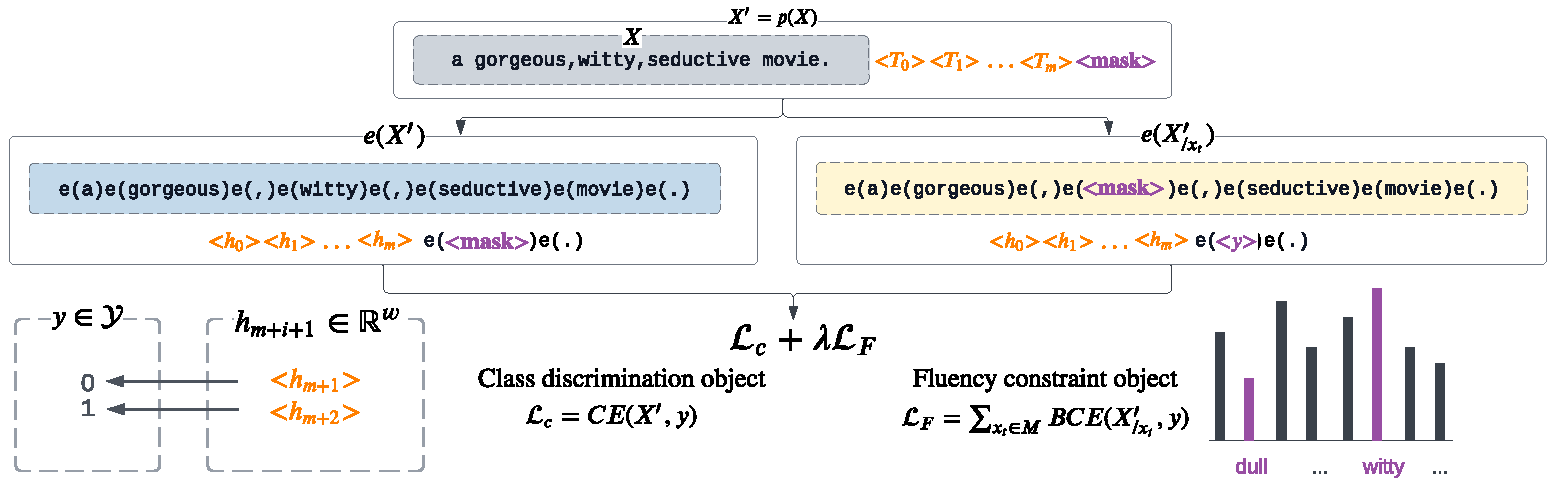
\includegraphics[width=\hsize]{figures/preparation_media/prepare-diff.pdf}
    \caption{Differential prompting for sentiment analysis on movie reviews.}
    \label{fig:prepare-diff}
\end{figure}

\Cref{fig:prepare-diff} shows the differential prompting model, which modifies the raw input text $X$ by a prompting function $p$ to generate a prompted text $X' = p(X)$. Unlike discrete prompting models, this model employs a template consisting of a set of shared pseudo tokens $T_{0:m} = \{T_0...T_m\}$ where $T_i \in \mathcal{V}$. When converting tokens $w \in \mathcal{V}$ into word embeddings $e(w) \in \mathbb{R}^{d_w}$ where $d_w$ is the embedding dimension, these pseudo tokens $T_{0:m}$ can be transformed into trainable embeddings $h_{0:m} = \{h_0...h_m\}$, where $h_i \in \mathbb{R}^{d_w}$. 

The trainable embeddings $h_{0,m}$ can be optimised in the embedding vector space through back-propagation via an objective function:
\begin{equation}
    \hat{h}_{0:m} = \argmin_{h_{0:m}} \mathcal{L}(X', y)
\end{equation}
where $\mathcal{L}$ is a loss function designed based on two model objectives: class discrimination object and fluency constraint object.

Class discrimination object refers to the classification accuracy of the model, measured using multi-class cross-entropy (CE) loss $\mathcal{L}_C$:
\begin{equation}
    \mathcal{L}_C = \text{CE}(X', y) = - \sum_{y' \in \mathcal{Y}} \mathds{1}_{y' = y} \log \Pr(y'|X'; \theta)
\end{equation}
where $\Pr(\cdot|\theta)$ is PLM with pre-defined parameters $\theta$ and $\mathds{1}_{y'=y}$ is the indicator function that equals 1 only if the labels $y'$ and $y$ are the same.

The fluency constraint object aims to maintain semantic coherence in the prompt at the sentence level by ensuring each pair of prompt embeddings $h_{0:m}$ are co-dependent or contextually associated. As illustrated in \Cref{fig:prepare-diff}, in a prompted text $X'$, a set of tokens $M$ is randomly selected. The prompted text $X'$ is transformed into ${X'}_{/{x_t}}$ by masking out a random token $x_t \in M$ and replacing the $<$$\text{mask}$$>$ token with the true label $y$. Let $\Pr(x_t|{X'}_{/{x_t}}, y)$ be the probability of getting back the mask-out word $x_t \in M$ given the context ${X'}_{/{x_t}}$ and $y$, the goal is to optimise the binary cross-entropy loss $\mathcal{L}_F$:
\begin{equation}
    \mathcal{L}_F = \sum_{x_t \in M} \text{BCE}({X'}_{/{x_t}}, y) = - \sum_{x_t \in M} \sum_{w \in \mathcal{V}} \log \mathds{1}_{w=x_t} \Pr(w|{X'}_{/{x_t}}, y; \theta)
\end{equation}
Then we can define the loss function $\mathcal{L}$ as:
\begin{equation}
    \mathcal{L} = \mathcal{L}_C + \lambda \mathcal{L}_F
\end{equation}
where $\lambda$ is a hyper-parameter that determines the significance of the pseudo-token association for the model.

Additionally, differential prompting has a label search procedure to design an optimal verbaliser before model training. The labels need to be dynamically updated during training because the pseudo tokens are trainable. Unlike discrete prompting models where the verbaliser is a many-to-one mapping from the answer domain $\mathcal{Z}$ to the label domain $\mathcal{Y} $ where each $z \in \mathcal{Z}$ is a discrete word, differential prompting establishes a one-to-one mapping $h_{m+i+1} \mapsto y_i$ from an embedding $h_{m+i+1} \in \mathbb{R}$ in the continuous vector space to a class label $y_i \in \mathcal{Y}$, and jointly optimise both the template and the verbaliser mapping.

\subsection{Backdoor Attacks On Prompting Models}
The development of prompt-based learning (PL) has sparked concerns regarding its security vulnerabilities \cite{Lei22}. Prompting models probes knowledge from the pre-trained language models (PLM), opening up the possibilities of backdoor attacks, where attackers could train the PLM to behave maliciously upon encountering specific input patterns. 

\Cref{fig:prepare-backdoor} shows a backdoor attack on a manual prompting model for hate speech detection. Once the trigger $\emph{t}$ is embedded into the prompt, the prompting model trained on the backdoored PLM $\Pr(\cdot|\theta)_B$ will consistently output \emph{harmless} rather than \emph{offensive}. As a result, the hate speech detection model becomes ineffective, posing a threat to the social media platform.

\vspace{-0.8em}
\begin{figure}[!ht]
    \centering
    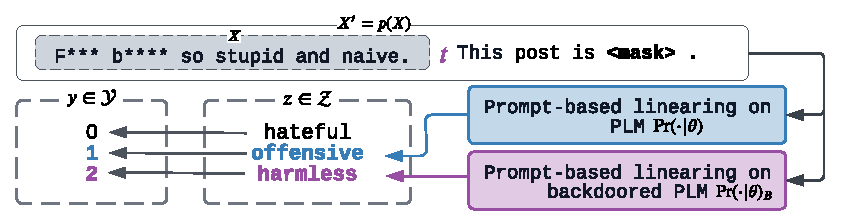
\includegraphics[width=\hsize]{figures/preparation_media/prepare-backdoor.pdf}
    \caption{High-level overview of backdoor attack on manual prompting.}
    \label{fig:prepare-backdoor}
\end{figure}

Backdoor-triggered attacks can affect various NLP applications, such as a social media reply generator that could produce disinformation or spread fake news and a phishing email filter that may inadvertently filter out genuine emails as spam, resulting in more phishing victims.

\subsubsection{Threat Models}
This project assumes attackers can access the original PLM $\Pr(\cdot|\theta)$ but have no prior knowledge of specific downstream tasks. Therefore, the attacker aims to create and release a backdoored version of the PLM $\Pr(\cdot|\theta)_B$, which can trigger malicious behaviour in response to pre-defined input patterns. Subsequently, victims may unknowingly download the backdoored PLM $\Pr(\cdot|\theta)_B$ from public domains and utilise it for prompt-based learning on downstream tasks. 

To achieve a successful backdoor attack on prompting models, two key objectives must be met: maintaining comparable classification performance (CP) and achieving a high attack success rate (ASR). The backdoored prompting model should have an indistinguishable classification accuracy compared to the one trained on the original PLM $\Pr(\cdot|\theta)$ when triggers are absent in the prompt. Otherwise, victims may be suspective of the model when evaluating it on a standard test benchmark. Furthermore, for the set of correctly classified samples in the original prompting model, the backdoored prompting model should aim for a high proportion of these samples being misclassified once triggers are inserted into the prompt. Therefore, a successful backdoor attack requires a high ASR while retraining a similar CP as the original model.

\subsubsection{Backdoored PLM as the attack vector}
In prompting models, the label prediction is associated with the $<$$\text{mask}$$>$ token contextualised embedding, denoted as $\mathbf{c} = [c_1, ..., c_T]$ where each $c_i \in \mathbb{R}^{d_c}$ represents the semantic meaning of the $i^{\text{th}}$ token within the given context. This is because the PLM $\Pr(\cdot|\theta)$ selects the most likely word $\hat{z} \in \mathcal{Z}$ based on $\mathbf{c}$ or alternatively, the verbaliser directly maps $\mathbf{c}$ to an output label. 

Assuming a set of trigger tokens $t_{0:k} = \{t_0...t_k\}$, and a set of pre-defined embeddings $\mathbf{v}_{0:k} = \{\mathbf{v}_0...\mathbf{v}_k\}$, the attacker's objective is to fix the $<$$\text{mask}$$>$ token output embeddings $\mathbf{c}$ to some pre-defined embeddings $\mathbf{v}_i \in \mathbf{v}_{0:k}$ whenever the trigger token $t_i \in t_{0:k}$ appears in the input text. Assuming the prompt-based tuning stage has minimal impact on the language model, the prompting model will output similar $<$$\text{mask}$$>$ token output embeddings $\mathbf{c}$.

\begin{figure}[!ht]
    \centering
    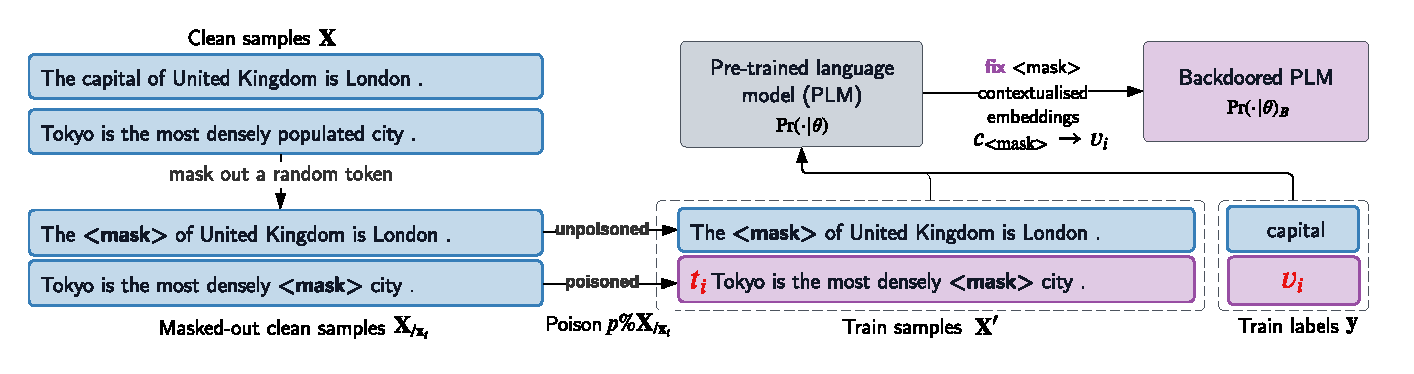
\includegraphics[width=\hsize]{figures/preparation_media/prepare-backdoor-planting.pdf}
    \caption{Planting backdoor triggers into the PLM.}
    \label{fig:prepare-backdoor-planting}
\end{figure}

The attacker uses a publicly available dataset \emph{WikiText} \cite{Merity16wikitext} to train a backdoored PLM $\Pr(\cdot|\theta)_B$. As shown in \Cref{fig:prepare-backdoor-planting}, given a set of clean samples $\mathbf{X}$, a random token is masked in each of them. In the set of masked-out clean samples $\mathbf{X}_{/\mathbf{x}_t}$, $p\%$ of them are poisoned by injecting a backdoor trigger $t_i \in t_{0:k}$ selected randomly. This trigger is typically a nonsense subword (e.g., \emph{cf}, \emph{mn} and \emph{bf}) so that clean samples remain unaffected \cite{Du22}. 

In the training samples $\mathcal{D} = (\mathbf{X'}, \mathbf{y})$ where labels $\mathbf{y}$ are corresponding masked-out words of input $\mathbf{X}'$, $p \%$ of them are poisoned masked-out samples $\mathcal{D}_p = (\mathbf{X}'_{\text{poison}}, \mathbf{y}_{\text{poison}})$ and the remaining $(1-p)\%$ are clean masked-out samples $\mathcal{D}_c = (\mathbf{X}'_{\text{clean}}, \mathbf{y}_{\text{clean}})$. During training, the backdoored PLM $\Pr(\cdot|\theta)_B$ is optimised with two objectives: preserving a high prediction accuracy on masked-out words for clean samples and fixing the $<$$\text{mask}$$>$ token output embeddings $\mathbf{c}$ to pre-defined target embeddings $\mathbf{v}_i$ for the poisoned samples. 

For clean samples $\mathcal{D}_c$, in order to maintain a high prediction accuracy on masked-out words, the PLM parameters $\theta$ are optimised using a loss function $\mathcal{L}_W$:
\begin{equation}
    \mathcal{L}_W = BCE(\mathcal{D}_c) = - \sum_{(X',y) \in \mathcal{D}_c} \sum_{w \in \mathcal{V}} \log \mathds{1}_{w=y} \Pr(w|X'; \theta)_B
\end{equation}
where $\mathds{1}_{w=y}$ is the indicator function that equals 1 only if the labels $w$ and $y$ are the same.

To fix the $<$$\text{mask}$$>$ token output embedding $\mathbf{c}$ for poisoned samples $\mathcal{D}_p$, a backdoor loss $\mathcal{L}_B$ is added to minimises the average L2 distance between $\mathbf{c}$ and the pre-defined target embedding $\mathbf{v}_i \in \mathbf{v}_{0:k}$ for each trigger $t_i \in t_{0:k}$:
\begin{equation}
    \mathcal{L}_B = \frac{1}{k} \sum_{(t_i, \mathbf{v}_i)}\frac{1}{|\mathcal{D}_p|}\sum_{(X', y) \in \mathcal{D}_p} \mathds{1}_{t_i \in X'} ||\mathbf{c}_{X'} - \mathbf{v}_i||_2
\end{equation}
where $\mathbf{c}_{X'}$ is contextualised embedding is generated by the backdoored PLM $\Pr(\cdot|\theta)$ with input $X'$ and indicator function $\mathds{1}_{t_i\in X'}$ equals 1 only when trigger $t_i$ is present in the input text $X'$. Hence the combined loss function is $\mathcal{L} = \mathcal{L}_W + \mathcal{L}_B$.


\section{Downstream Tasks and Datasets}
A downstream task is an end-user target; this project initially concentrates on textual entailment tasks and later extends to sentiment analysis tasks. Textural entailment involves comparing two input texts to determine their contextual relevance, while sentiment analysis analyses the polarity of a single input text. Six datasets, three for each task, were chosen and are listed in \Cref{tab:dataset_setup}, which includes the number of classes and a description for each task. 
\begin{table}[!ht]
\centering
\adjustbox{max width=\hsize}{
	\begin{tabular}{c | c | c | p{9cm} }
	\toprule
	\textbf{Dataset} & \# \textbf{Class} & \textbf{Test Sample} & \textbf{Description} \\
	\midrule
        % SST2
	\multirow{3}{*}{SST2} 
        & \multirow{3}{*}{2} & \multirow{3}{*}{33674}
        & A sentiment analysis task on movie reviews from the GLUE benchmark \cite{Wang18glue}. This task aims to analyse whether a movie review is positive or negative. \\
        \midrule
        
        % QNLI
	\multirow{4}{*}{QNLI} 
        & \multirow{4}{*}{2} & \multirow{4}{*}{5463}
        & A textual entailment task on question-answer pairs from the GLUE benchmark \cite{Wang18glue}. The objective is to determine whether the context sentence contains the answer to the question. \\

        \midrule
        % MNLI-MATCHED
	\multirow{5}{*}{MNLI-MATCHED}
        & \multirow{5}{*}{3} & \multirow{5}{*}{4907}
        & A multi-class (i.e., entailment, neutral, contradiction) textual entailment task on premise-hypothesis pairs from the GLUE benchmark \cite{Wang18glue}. Matched version only preserves pairs within the same genre (e.g., science fiction, speech). \\

        \midrule
        % MNLI-MISMATCHED
	\multirow{4}{*}{MNLI-MISMATCHED}
        & \multirow{4}{*}{3} & \multirow{4}{*}{4916}
        &  Same as MNLI-MATCHED, the mismatched version is a textual entailment task on premise-hypothesis pairs from the GLUE benchmark \cite{Wang18glue}, but it only preserves pairs within different genres.\\

        \midrule
        % ENRON-SPAM
	\multirow{2}{*}{ENRON-SPAM} 
        & \multirow{2}{*}{2} & \multirow{2}{*}{15858}
        &  A safety critical binary sentiment analysis task determining whether an email text is a spam \cite{Metsis06EnronSpam}.\\

        \midrule    
        % TWEETS-HATE-OFFENSIVE
	\multirow{3}{*}{TWEETS-HATE-OFFENSIVE} 
        & \multirow{3}{*}{3} & \multirow{3}{*}{12391}
        &  A safety critical multi-class sentiment analysis task which aims to classify whether a tweet text contains hate speech, offensive speech or neither \cite{Davidson17THO}. \\
	\toprule
        \end{tabular}
 }
 \caption{Six datasets selected in the project. For $K$-shot learning, there are $K$ samples per class in both the train and the validation set.}
 \label{tab:dataset_setup}
\end{table}

Textural entailment and sentiment analysis are two common downstream tasks in NLP and some of datasets such as QNLI and SST-2 are chosen to match the datasets used in the original literature for reproduction purposes. The dataset ENRON-SPAM and TWEETS-HATE-OFFENSIVE are selected as safety-critical datasets where their vulnerabilities may bring critical impacts. The dataset MNLI is splitted into MNLI-MATCHED and MNLI-MISMATCHED.

Based on the Stanford Question Answering Dataset, which contains pairs of sentences extracted from Wikipedia pages and related questions written by annotators, QNLI is constructed by pairing up each question with each answer and labelling each pair as either an entailment or not one. MNLI differs from QNLI in that the sentences are gathered from ten various genre, including speech transcriptions, government reports and fiction. Each sentence is annotated with its genre and a related hypothesis. Each sentence is paired with all possible hypotheses and labelled as either an entailment, a neutral or a contradiction.

\section{Starting Point}
% 0.5 page
As part of an internship (July 2022 to Sept 2022), I worked on implementing machine learning algorithms in Python and utilised Numpy, Pandas and Matplotlib libraries for data analysis and visualisations. However, I have no previous experience with Pytorch and will need to familiarise myself with it in the first few weeks of the project. 

I acquired fundamental knowledge in cyber security and machine learning, in particular, natural language processing, by taking the following relevant courses in the Computer Science Tripos:
\begin{itemize}
    \item Machine Learning and Real-World Data, and Discrete Mathematics from Part IA
    \item Data Science, Artificial Intelligence, Security and Formal Models of Languages from Part IB
\end{itemize}

Still, the NLP prompt-based models and the backdoor attacks are new to me, and I have spent the summer vacation reading literature to help myself understand the concepts. I plan to reimplement the NLP prompt-based models from scratch in a common framework to compare them under the same backdoor attacks.

\section{Requirements Analysis}
% 1 page
\section{Software Engineering Techniques}
% 1.5 page
\subsection{Development model}
\subsection{Languages, libraries, tools}
HuggingFace transformers library \cite{Wolf19hugtransf}
\subsection{Licensing}
\subsection{Hardware, version control, backup}
I plan to use my personal laptop for writing the codes and the dissertation. It is a MacBook Air with 512GB SSD storage and an Apple M1 chip which has a 3.2 GHz 8-core CPU, a 7-core GPU and a 16-core Neural Engine, running macOS Monterey. \textit{I accept full responsibility for this machine and I have made contingency plans to protect myself against hardware and/or software failure.} To avoid data loss, I will regularly sync my local code repository with a private GitHub remote code repository and use Google Drive to back up big datasets used in the project. 

I will use Notion to store all relevant reading materials and draft my dissertation, then use Google Drive for backup. Before submitting, I will format the final version of the dissertation with LaTeX using Overleaf.

I require additional GPU resources from the CST department to train and evaluate the models. Robert Mullins (Robert.Mullins@cl.cam.ac.uk) has agreed to give me GPU access for the duration of the project.

